\documentclass[12pt,a4paper]{article}

\usepackage[utf8]{inputenc}
\usepackage[T2A]{fontenc}
\usepackage[russian]{babel}
\usepackage{amsmath}
\usepackage{amssymb}
\usepackage{array}
\usepackage{booktabs}
\usepackage{caption}
\usepackage{enumitem}
\usepackage{fancyhdr}
\usepackage{float}
\usepackage{geometry}
\usepackage{graphicx}
\usepackage{hyperref}
\usepackage{indentfirst}
\usepackage{listings}
\usepackage{longtable}
\usepackage{multirow}
\usepackage{tikz}
\usepackage{xcolor}

\geometry{left=30mm,right=15mm,top=20mm,bottom=20mm}
\setlength{\parindent}{1.25cm}
\linespread{1.2}
\pagestyle{fancy}
\fancyhf{}
\fancyfoot[C]{\thepage}
\renewcommand{\headrulewidth}{0pt}
\hypersetup{hidelinks}

\captionsetup{justification=centering}

\usetikzlibrary{arrows.meta,positioning,shapes.geometric,shapes.symbols}

\definecolor{codebg}{RGB}{248,248,248}
\definecolor{codeframe}{RGB}{215,215,215}
\definecolor{codekw}{RGB}{0,76,153}
\definecolor{codestr}{RGB}{163,21,21}
\definecolor{codecomment}{RGB}{0,128,0}

\lstdefinelanguage{JavaScript}{
  morekeywords={const,let,var,function,return,if,else,for,while,throw,new,export,import,from},
  sensitive=true,
  morecomment=[l]{//},
  morestring=[b]",
  morestring=[b]',
}

\lstset{
  language=JavaScript,
  basicstyle=\ttfamily\small,
  keywordstyle=\color{codekw}\bfseries,
  stringstyle=\color{codestr},
  commentstyle=\color{codecomment},
  backgroundcolor=\color{codebg},
  frame=single,
  rulecolor=\color{codeframe},
  numbers=left,
  numberstyle=\tiny,
  stepnumber=1,
  breaklines=true,
  showstringspaces=false,
  tabsize=2,
  columns=fullflexible,
  keepspaces=true
}

\newcolumntype{C}[1]{>{\centering\arraybackslash}p{#1}}

\tikzset{
  flowstart/.style = {
    ellipse,
    draw,
    align=center,
    minimum width=26mm,
    minimum height=8mm
  },
  flowio/.style = {
    trapezium,
    trapezium left angle=70,
    trapezium right angle=110,
    draw,
    align=center,
    minimum width=34mm,
    minimum height=9mm
  },
  flowproc/.style = {
    rectangle,
    draw,
    align=center,
    rounded corners=1mm,
    minimum width=42mm,
    minimum height=9mm
  },
  flowdecision/.style = {
    diamond,
    draw,
    aspect=2.1,
    align=center,
    inner sep=1pt,
    minimum width=32mm,
    minimum height=10mm
  },
  flowarrow/.style = {
    -{Latex[length=2.5mm]},
    thick
  }
}

\begin{document}

\pagenumbering{gobble}
\hypersetup{pageanchor=false}
\begin{titlepage}
  \thispagestyle{empty}
  \begin{center}
    {\small Федеральное государственное автономное образовательное учреждение высшего образования\\
    «Национальный исследовательский университет ИТМО»}\\[0.8em]
    {\small Факультет программной инженерии и компьютерной техники}

    \vfill

    {\Large\textbf{Лабораторная работа №2}}\\[0.6em]
    {\large по курсу «Вычислительная математика»}\\[0.6em]
    {\large Вариант 19}

    \vfill

    \begin{flushright}
      \begin{tabular}{l}
        Выполнил:\\
        Якименко Владислав Игоревич, Р3213\\[0.8em]
        Проверила:\\
        Малышева Татьяна Алексеевна
      \end{tabular}
    \end{flushright}

    \vfill

    Санкт-Петербург --- 2026
  \end{center}
\end{titlepage}
\clearpage
\hypersetup{pageanchor=true}

\tableofcontents
\thispagestyle{empty}
\clearpage
\pagenumbering{arabic}

\section{Вычислительная реализация задачи}

\subsection{Часть. Решение нелинейного уравнения}

\textbf{Задание:}
\begin{enumerate}[label=\arabic*., leftmargin=1.2cm]
  \item Отделить корни заданного нелинейного уравнения графически.
  \item Определить интервалы изоляции корней.
  \item Уточнить корни нелинейного уравнения с точностью $\varepsilon = 10^{-2}$.
  \item Вычисления оформить в виде таблиц.
\end{enumerate}

\textbf{Уравнение:}
\[
f(x) = 2x^3 - 1.89x^2 - 5x + 2.34
\]

\textbf{Производная:}
\[
f'(x) = 6x^2 - 3.78x - 5
\]

\textbf{Вторая производная:}
\[
f''(x) = 12x - 3.78
\]

\subsubsection{Отделение корней (графический метод)}

Построим график функции $f(x)$ на интервале $[-3; 3]$.

\begin{figure}[H]
  \centering
  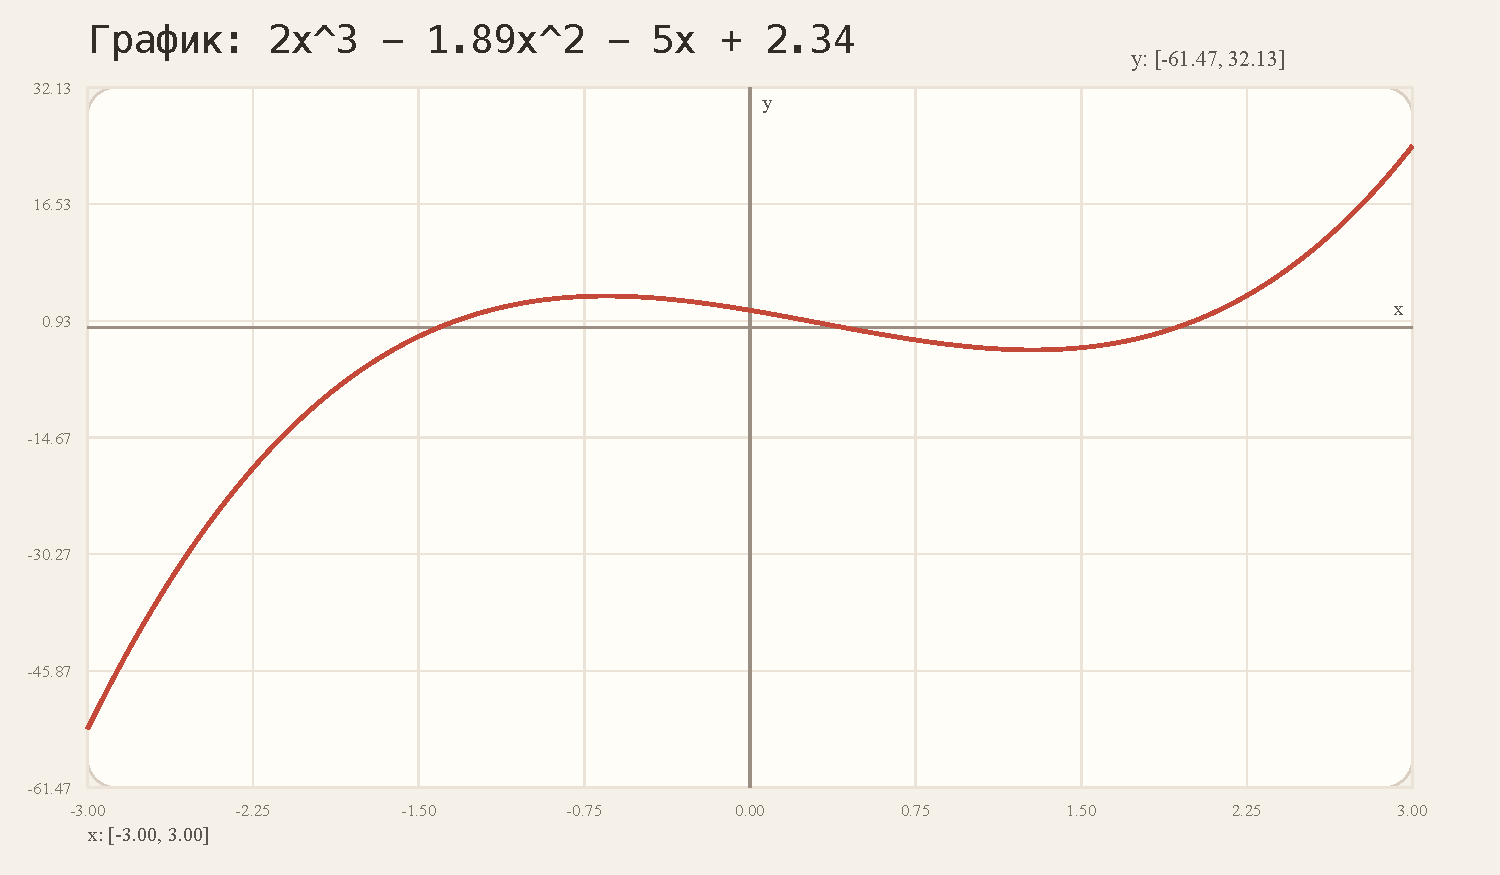
\includegraphics[width=0.96\textwidth]{output/latex-assets/report-variant19-equation.pdf}
  \caption{График функции $f(x) = 2x^3 - 1.89x^2 - 5x + 2.34$}
\end{figure}

По графику видно, что уравнение имеет три действительных корня:
\[
x_1 \approx -1.41,\qquad x_2 \approx 0.43,\qquad x_3 \approx 1.93.
\]

\subsubsection{Интервалы изоляции корней}

Для левого корня выберем интервал $[-1.50;\,-1.25]$:
\[
f(-1.50) = -1.162 < 0,\qquad f(-1.25) = 1.731 > 0.
\]

Для центрального корня выберем интервал $[0.00;\,1.00]$:
\[
f(0.00) = 2.340 > 0,\qquad f(1.00) = -2.550 < 0.
\]

Для правого корня выберем интервал $[1.50;\,2.00]$:
\[
f(1.50) = -2.475 < 0,\qquad f(2.00) = 0.780 > 0.
\]

Таким образом, на каждом из выбранных интервалов происходит смена знака функции, значит корень на интервале существует.

\subsubsection[Уточнение корней (eps = 10\textasciicircum -2)]{Уточнение корней ($\varepsilon = 10^{-2}$)}

В вычислительной части использованы методы, которые уже подготовлены в проекте для отчёта:
\begin{center}
  \begin{tabular}{C{30mm}C{48mm}C{42mm}}
    \toprule
    Корень & Интервал изоляции & Метод \\
    \midrule
    Левый $x_1$ & $[-1.50;\,-1.25]$ & половинного деления \\
    Центральный $x_2$ & $[0.00;\,1.00]$ & секущих \\
    Правый $x_3$ & $[1.50;\,2.00]$ & простой итерации \\
    \bottomrule
  \end{tabular}
\end{center}

\paragraph{Левый корень. Метод половинного деления.}
Рабочая формула:
\[
x = \frac{a+b}{2}.
\]

Критерий остановки:
\[
|b-a| \le \varepsilon \quad \text{или} \quad |f(x)| \le \varepsilon.
\]

Получено:
\[
x_1 \approx -1.410156,\qquad f(x_1) \approx 0.024133,\qquad n = 6.
\]

\begin{table}[H]
  \centering
  \caption{Метод половинного деления для левого корня}
  \begin{tabular}{C{10mm}C{18mm}C{18mm}C{18mm}C{18mm}C{18mm}C{18mm}C{18mm}}
    \toprule
    № & $a$ & $b$ & $x$ & $f(a)$ & $f(b)$ & $f(x)$ & $|b-a|$ \\
    \midrule
    1 & -1.500 & -1.250 & -1.375 & -1.162 & 1.731 & 0.442 & 0.250 \\
    2 & -1.500 & -1.375 & -1.438 & -1.162 & 0.442 & -0.319 & 0.125 \\
    3 & -1.438 & -1.375 & -1.406 & -0.319 & 0.442 & 0.072 & 0.063 \\
    4 & -1.438 & -1.406 & -1.422 & -0.319 & 0.072 & -0.121 & 0.031 \\
    5 & -1.422 & -1.406 & -1.414 & -0.121 & 0.072 & -0.024 & 0.016 \\
    6 & -1.414 & -1.406 & -1.410 & -0.024 & 0.072 & 0.024 & 0.008 \\
    \bottomrule
  \end{tabular}
\end{table}

\paragraph{Центральный корень. Метод секущих.}
Рабочая формула:
\[
x_{k+1} = x_k - \frac{f(x_k)(x_k - x_{k-1})}{f(x_k)-f(x_{k-1})}.
\]

Критерий остановки:
\[
|x_{k+1} - x_k| \le \varepsilon.
\]

Получено:
\[
x_2 \approx 0.430001,\qquad f(x_2) \approx -0.000454,\qquad n = 3.
\]

\begin{table}[H]
  \centering
  \caption{Метод секущих для центрального корня}
  \begin{tabular}{C{10mm}C{20mm}C{20mm}C{20mm}C{24mm}C{26mm}}
    \toprule
    № & $x_{i-1}$ & $x_i$ & $x_{i+1}$ & $f(x_{i+1})$ & $|x_{i+1}-x_i|$ \\
    \midrule
    1 & 0.000 & 1.000 & 0.479 & -0.266 & 0.521 \\
    2 & 1.000 & 0.479 & 0.418 & 0.067 & 0.061 \\
    3 & 0.479 & 0.418 & 0.430 & -0.000 & 0.012 \\
    \bottomrule
  \end{tabular}
\end{table}

\paragraph{Правый корень. Метод простой итерации.}
Использована итерационная форма
\[
x_{k+1} = \varphi(x_k) = x_k + \lambda f(x_k),
\]
где коэффициент сжатия
\[
q = \max |\varphi'(x)| = 0.752622 < 1.
\]

Получено:
\[
x_3 \approx 1.927069,\qquad f(x_3) \approx -0.001336,\qquad n = 4.
\]

\begin{table}[H]
  \centering
  \caption{Метод простой итерации для правого корня}
  \begin{tabular}{C{10mm}C{18mm}C{18mm}C{24mm}C{24mm}C{28mm}}
    \toprule
    № & $x_i$ & $x_{i+1}$ & $\varphi(x_{i+1})$ & $|x_{i+1}-x_i|$ & Оценка погрешности \\
    \midrule
    1 & 1.750 & 1.879 & 1.919 & 0.129 & 0.393 \\
    2 & 1.879 & 1.919 & 1.926 & 0.040 & 0.122 \\
    3 & 1.919 & 1.926 & 1.927 & 0.007 & 0.021 \\
    4 & 1.926 & 1.927 & 1.927 & 0.001 & 0.003 \\
    \bottomrule
  \end{tabular}
\end{table}

\paragraph{Итог по уравнению.}
\begin{center}
  \begin{tabular}{C{28mm}C{42mm}C{22mm}C{22mm}C{18mm}}
    \toprule
    Корень & Метод & $x^*$ & $f(x^*)$ & Итераций \\
    \midrule
    Левый & половинного деления & -1.410 & 0.024 & 6 \\
    Центральный & секущих & 0.430 & -0.000 & 3 \\
    Правый & простой итерации & 1.927 & -0.001 & 4 \\
    \bottomrule
  \end{tabular}
\end{center}

\subsection{Часть. Решение системы нелинейных уравнений}

\textbf{Задание:}
\begin{enumerate}[label=\arabic*., leftmargin=1.2cm]
  \item Отделить корни заданной системы нелинейных уравнений графически.
  \item Привести систему к виду, пригодному для итерационного процесса.
  \item Проверить условие сходимости итерационного процесса.
  \item Уточнить решение системы с точностью $\varepsilon = 10^{-2}$.
  \item Вычисления оформить в виде таблиц.
\end{enumerate}

\textbf{Система:}
\[
\begin{cases}
\sin(y - 1) + x = 1.3,\\
y - \sin(x + 1) = 0.8.
\end{cases}
\]

\textbf{Метод:} простая итерация.

\subsubsection{Отделение корней (графический метод)}

Построим график кривых $F_1(x,y)=0$ и $F_2(x,y)=0$ на области, содержащей точку пересечения.

\begin{figure}[H]
  \centering
  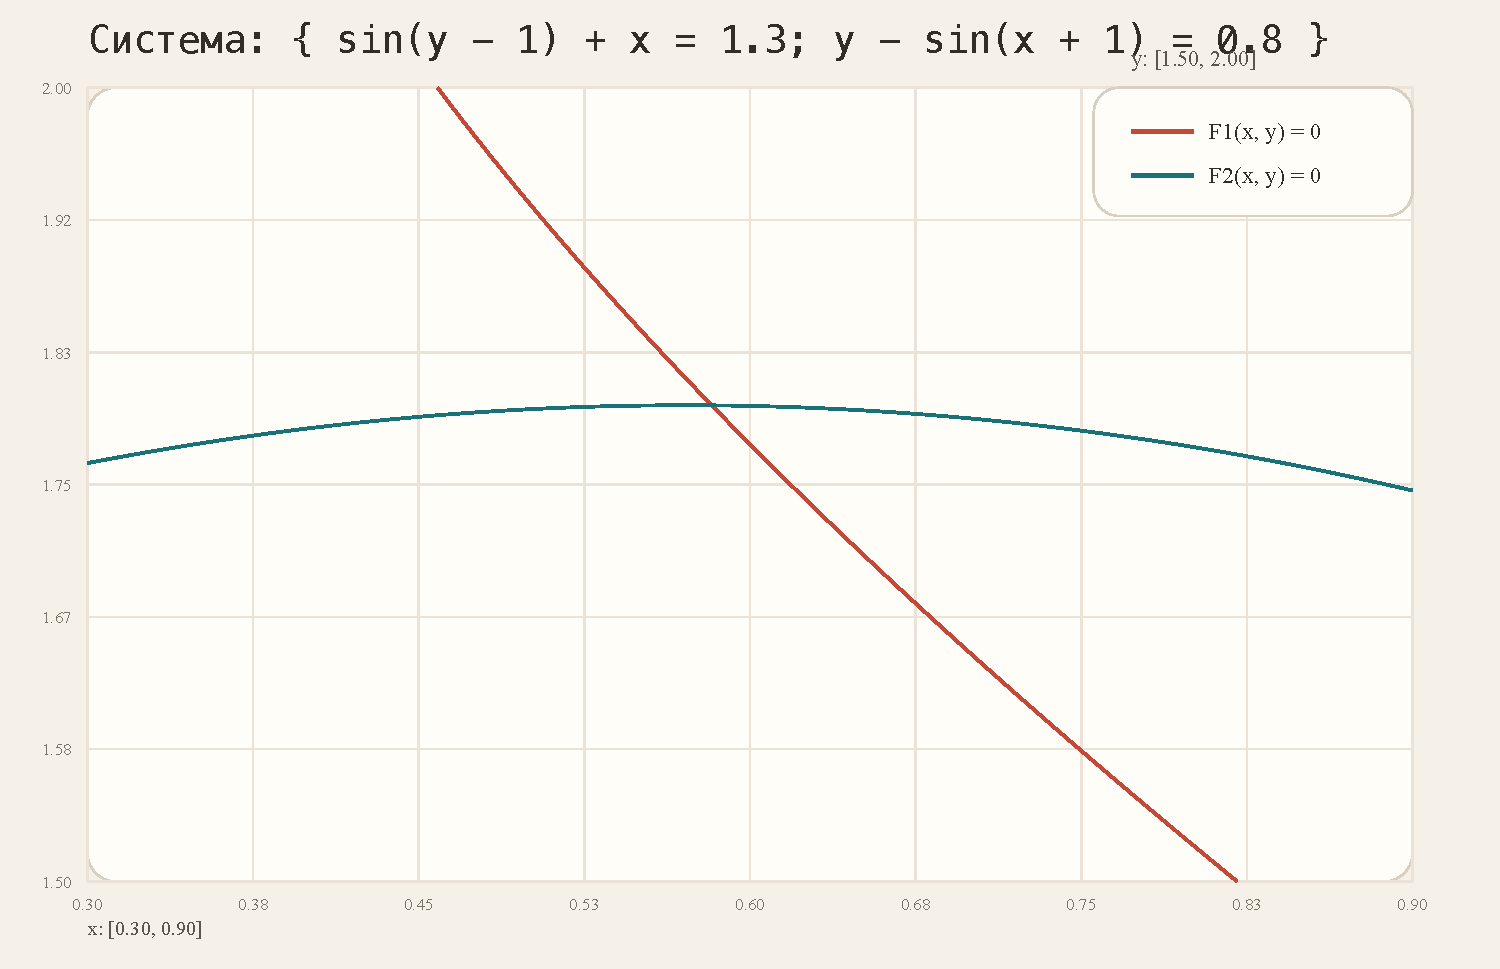
\includegraphics[width=0.96\textwidth]{output/latex-assets/report-variant19-system.pdf}
  \caption{Графическое отделение корня системы варианта 19}
\end{figure}

По графику видно, что точка пересечения находится вблизи
\[
(x_0,\;y_0) \approx (0.58,\;1.80).
\]

\subsubsection[Приведение к виду x = phi1(x,y), y = phi2(x,y)]{Приведение к виду $x = \varphi_1(x,y)$, $y = \varphi_2(x,y)$}

Для метода простой итерации систему запишем в виде
\[
\begin{cases}
x = 1.3 - \sin(y - 1),\\
y = 0.8 + \sin(x + 1).
\end{cases}
\]

Тогда
\[
\Phi(x,y) =
\begin{pmatrix}
1.3 - \sin(y - 1)\\
0.8 + \sin(x + 1)
\end{pmatrix}.
\]

\subsubsection{Проверка условия сходимости}

Матрица Якоби отображения $\Phi(x,y)$ имеет вид:
\[
D\Phi(x,y)=
\begin{pmatrix}
0 & -\cos(y - 1)\\
\cos(x + 1) & 0
\end{pmatrix}.
\]

На прямоугольнике
\[
[0.50;\,0.65] \times [1.75;\,1.85]
\]
получаем
\[
q = \max \|D\Phi(x,y)\|_{\infty} \approx 0.731689 < 1.
\]

Следовательно, достаточное условие сходимости метода простой итерации выполняется.

\subsubsection[Уточнение решения (eps = 10\textasciicircum -2)]{Уточнение решения ($\varepsilon = 10^{-2}$)}

Рабочие формулы:
\[
\begin{cases}
x_{k+1} = 1.3 - \sin(y_k - 1),\\
y_{k+1} = 0.8 + \sin(x_k + 1).
\end{cases}
\]

Получено:
\[
x^* \approx 0.583432,\qquad y^* \approx 1.799908.
\]

Невязки:
\[
F_1(x^*,y^*) \approx 0.000724,\qquad F_2(x^*,y^*) \approx -0.000013.
\]

\begin{table}[H]
  \centering
  \caption{Метод простой итерации для системы варианта 19}
  \begin{tabular}{C{10mm}C{18mm}C{18mm}C{18mm}C{18mm}C{22mm}C{28mm}}
    \toprule
    № & $x_i$ & $y_i$ & $x_{i+1}$ & $y_{i+1}$ & max diff & Оценка погрешности \\
    \midrule
    1 & 0.500 & 1.750 & 0.618 & 1.797 & 0.118 & 0.323 \\
    2 & 0.618 & 1.797 & 0.584 & 1.799 & 0.034 & 0.093 \\
    3 & 0.584 & 1.799 & 0.583 & 1.800 & 0.001 & 0.003 \\
    \bottomrule
  \end{tabular}
\end{table}

\paragraph{Итог по системе.}
\[
(x^*, y^*) \approx (0.583,\;1.800), \qquad n = 3.
\]

\clearpage
\section{Программная реализация}

В программной части варианта 19 реализованы методы $2$, $3$, $5$ и $6$ из задания:
\begin{itemize}[leftmargin=1.2cm]
  \item метод хорд;
  \item метод Ньютона;
  \item метод простой итерации для одного уравнения;
  \item метод Ньютона для системы нелинейных уравнений.
\end{itemize}

Проект написан на JavaScript. Консольная часть запускается через Node.js, а для визуализации дополнительно сделан GUI в браузере. Программа умеет принимать входные данные с клавиатуры или из JSON-файла, проверяет корректность интервала изоляции, строит графики и выводит историю итераций.

\subsection{Блок-схемы алгоритмов}

\subsubsection{Блок-схема метода хорд}

\begin{figure}[H]
  \centering
  \begin{tikzpicture}[node distance=9mm]
    \node[flowstart] (start) {Начало};
    \node[flowio, below=of start] (input) {Ввод $f(x)$,\\$[a,b]$, $\varepsilon$};
    \node[flowproc, below=of input] (choose) {Выбрать фиксированный\\и подвижный конец};
    \node[flowproc, below=of choose] (calc) {Вычислить $x_{next}$\\по формуле хорд};
    \node[flowdecision, below=11mm of calc] (check) {$|x_{next}-x| \le \varepsilon$\\или $|f(x_{next})| \le \varepsilon$?};
    \node[flowproc, below left=12mm and 16mm of check] (update) {$x := x_{next}$};
    \node[flowio, below right=12mm and 16mm of check] (output) {Вывод $x_{next}$,\\$f(x_{next})$, $n$};
    \draw[flowarrow] (start) -- (input);
    \draw[flowarrow] (input) -- (choose);
    \draw[flowarrow] (choose) -- (calc);
    \draw[flowarrow] (calc) -- (check);
    \draw[flowarrow] (check) -- node[above left] {нет} (update);
    \draw[flowarrow] (check) -- node[above right] {да} (output);
    \draw[flowarrow] (update.west) -| ++(-1.8,0) |- (calc.west);
  \end{tikzpicture}
  \caption{Блок-схема метода хорд с неподвижным концом}
\end{figure}

\subsubsection{Блок-схема метода Ньютона}

\begin{figure}[H]
  \centering
  \begin{tikzpicture}[node distance=9mm]
    \node[flowstart] (start) {Начало};
    \node[flowio, below=of start] (input) {Ввод $f(x)$, $f'(x)$,\\$[a,b]$, $\varepsilon$};
    \node[flowproc, below=of input] (init) {Выбрать начальное\\приближение $x_0$};
    \node[flowproc, below=of init] (calc) {$x_{next}=x-\dfrac{f(x)}{f'(x)}$};
    \node[flowdecision, below=11mm of calc] (check) {$|x_{next}-x| \le \varepsilon$\\или $|f(x_{next})| \le \varepsilon$?};
    \node[flowproc, below left=12mm and 16mm of check] (update) {$x := x_{next}$};
    \node[flowio, below right=12mm and 16mm of check] (output) {Вывод $x_{next}$,\\$f(x_{next})$, $n$};
    \draw[flowarrow] (start) -- (input);
    \draw[flowarrow] (input) -- (init);
    \draw[flowarrow] (init) -- (calc);
    \draw[flowarrow] (calc) -- (check);
    \draw[flowarrow] (check) -- node[above left] {нет} (update);
    \draw[flowarrow] (check) -- node[above right] {да} (output);
    \draw[flowarrow] (update.west) -| ++(-1.8,0) |- (calc.west);
  \end{tikzpicture}
  \caption{Блок-схема метода Ньютона}
\end{figure}

\subsubsection{Блок-схема метода простой итерации}

\begin{figure}[H]
  \centering
  \begin{tikzpicture}[node distance=8.5mm]
    \node[flowstart] (start) {Начало};
    \node[flowio, below=of start] (input) {Ввод $f(x)$,\\$[a,b]$, $\varepsilon$};
    \node[flowproc, below=of input] (phi) {Построить $\varphi(x)$,\\оценить $q$};
    \node[flowdecision, below=10mm of phi] (conv) {$q < 1$?};
    \node[flowio, right=24mm of conv] (noconv) {Вывод:\\нет сходимости};
    \node[flowproc, below=of conv] (init) {$x := \dfrac{a+b}{2}$};
    \node[flowproc, below=of init] (next) {$x_{next}:=\varphi(x)$};
    \node[flowproc, below=of next] (err) {Оценить\\погрешность};
    \node[flowdecision, below=11mm of err] (check) {Погрешность\\$\le \varepsilon$?};
    \node[flowproc, below left=12mm and 16mm of check] (update) {$x := x_{next}$};
    \node[flowio, below right=12mm and 16mm of check] (output) {Вывод $x_{next}$,\\$f(x_{next})$, $n$};
    \draw[flowarrow] (start) -- (input);
    \draw[flowarrow] (input) -- (phi);
    \draw[flowarrow] (phi) -- (conv);
    \draw[flowarrow] (conv) -- node[above] {нет} (noconv);
    \draw[flowarrow] (conv) -- node[right] {да} (init);
    \draw[flowarrow] (init) -- (next);
    \draw[flowarrow] (next) -- (err);
    \draw[flowarrow] (err) -- (check);
    \draw[flowarrow] (check) -- node[above left] {нет} (update);
    \draw[flowarrow] (check) -- node[above right] {да} (output);
    \draw[flowarrow] (update.west) -| ++(-1.8,0) |- (next.west);
  \end{tikzpicture}
  \caption{Блок-схема метода простой итерации}
\end{figure}

\subsubsection{Блок-схема метода Ньютона для системы}

\begin{figure}[H]
  \centering
  \begin{tikzpicture}[node distance=8.5mm]
    \node[flowstart] (start) {Начало};
    \node[flowio, below=of start] (input) {Ввод $x_0$, $y_0$,\\$\varepsilon$};
    \node[flowproc, below=of input] (fval) {Вычислить $F_1$, $F_2$\\и матрицу Якоби};
    \node[flowproc, below=of fval] (solve) {Решить систему\\для $\Delta x$, $\Delta y$};
    \node[flowproc, below=of solve] (next) {$x_{next}=x+\Delta x$,\\$y_{next}=y+\Delta y$};
    \node[flowdecision, below=11mm of next] (check) {$\max(|\Delta x|, |\Delta y|)\le\varepsilon$?};
    \node[flowproc, below left=12mm and 17mm of check] (update) {$x:=x_{next}$,\\$y:=y_{next}$};
    \node[flowio, below right=12mm and 17mm of check] (output) {Вывод $x^*$, $y^*$,\\невязок и $n$};
    \draw[flowarrow] (start) -- (input);
    \draw[flowarrow] (input) -- (fval);
    \draw[flowarrow] (fval) -- (solve);
    \draw[flowarrow] (solve) -- (next);
    \draw[flowarrow] (next) -- (check);
    \draw[flowarrow] (check) -- node[above left] {нет} (update);
    \draw[flowarrow] (check) -- node[above right] {да} (output);
    \draw[flowarrow] (update.west) -| ++(-2.0,0) |- (fval.west);
  \end{tikzpicture}
  \caption{Блок-схема метода Ньютона для системы}
\end{figure}

\subsection{Листинги программ}

Язык реализации: JavaScript (Node.js). Для вычислительных методов не используются сторонние библиотеки. Ниже приведены ключевые фрагменты из основных файлов с реализациями:
\begin{itemize}[leftmargin=1.2cm]
  \item \texttt{src/methods/equations.js};
  \item \texttt{src/methods/systems.js}.
\end{itemize}

\begin{lstlisting}[caption={Метод хорд с неподвижным концом (фрагмент \texttt{src/methods/equations.js})}]
export function chordFixed(equation, a, b, epsilon, maxIterations = 1000) {
  const history = [];
  const { fixed, moving } = chooseChordConfiguration(equation, a, b);
  const fFixed = equation.f(fixed);
  let current = moving;

  for (let iteration = 1; iteration <= maxIterations; iteration += 1) {
    const fCurrent = equation.f(current);
    const denominator = fFixed - fCurrent;
    if (Math.abs(denominator) < 1e-14) {
      throw new Error("...");
    }

    const next = current - (fCurrent * (fixed - current)) / denominator;
    const fNext = equation.f(next);
    const diff = Math.abs(next - current);

    history.push({
      iteration,
      fixed,
      moving: current,
      next,
      fFixed,
      fMoving: fCurrent,
      fNext,
      diff,
    });

    if (diff <= epsilon || Math.abs(fNext) <= epsilon) {
      return { method: "chord", root: next, fx: fNext, iterations: iteration, history };
    }
    current = next;
  }
  throw new Error("...");
}
\end{lstlisting}

\begin{lstlisting}[caption={Метод Ньютона (фрагмент \texttt{src/methods/equations.js})}]
export function newton(equation, a, b, epsilon, maxIterations = 1000) {
  const history = [];
  let current = chooseInitialByCurvature(equation, a, b);

  for (let iteration = 1; iteration <= maxIterations; iteration += 1) {
    const fx = equation.f(current);
    const dfx = equation.df(current);

    if (Math.abs(dfx) < 1e-14) {
      throw new Error("...");
    }

    const next = current - fx / dfx;
    const diff = Math.abs(next - current);
    const fNext = equation.f(next);

    history.push({ iteration, x: current, fx, dfx, next, diff, fNext });

    if (diff <= epsilon || Math.abs(fNext) <= epsilon) {
      return { method: "newton", root: next, fx: fNext, iterations: iteration, history };
    }
    current = next;
  }
  throw new Error("...");
}
\end{lstlisting}

\begin{lstlisting}[caption={Метод простой итерации (фрагмент \texttt{src/methods/equations.js})}]
export function simpleIterationEquation(equation, a, b, epsilon, maxIterations = 1000) {
  const { min, max, maxAbs } = estimateDerivativeStats(equation.df, a, b);
  const midpoint = (a + b) / 2;
  const signProbe = Math.sign(equation.df(midpoint)) || Math.sign(min + max) || 1;
  const lambda = -signProbe / maxAbs;
  const phi = (x) => x + lambda * equation.f(x);
  const q = estimateMaxAbs((x) => 1 + lambda * equation.df(x), a, b);

  if (q >= 1) {
    throw new Error("...");
  }

  let current = midpoint;
  for (let iteration = 1; iteration <= maxIterations; iteration += 1) {
    const next = phi(current);
    const diff = Math.abs(next - current);
    const estimatedError = q === 0 ? diff : (q / (1 - q)) * diff;

    if (estimatedError <= epsilon || Math.abs(equation.f(next)) <= epsilon) {
      return { method: "simpleIteration", root: next, fx: equation.f(next), iterations: iteration };
    }
    current = next;
  }
  throw new Error("...");
}
\end{lstlisting}

\begin{lstlisting}[caption={Метод Ньютона для системы (фрагмент \texttt{src/methods/systems.js})}]
export function newtonSystem(system, initial, epsilon, maxIterations = 100) {
  const history = [];
  let current = { ...initial };

  for (let iteration = 1; iteration <= maxIterations; iteration += 1) {
    const [f1, f2] = system.f(current.x, current.y);
    const jacobian = system.jacobian(current.x, current.y);
    const [dx, dy] = solveLinear2x2(jacobian, [-f1, -f2]);

    const next = {
      x: current.x + dx,
      y: current.y + dy,
    };
    const [nextF1, nextF2] = system.f(next.x, next.y);
    const errors = [Math.abs(dx), Math.abs(dy)];

    history.push({
      iteration,
      x: current.x,
      y: current.y,
      f1,
      f2,
      dx,
      dy,
      nextX: next.x,
      nextY: next.y,
      nextF1,
      nextF2,
    });

    if (maxAbs(errors) <= epsilon) {
      return { method: "newtonSystem", solution: next, residuals: [nextF1, nextF2], iterations: iteration };
    }
    current = next;
  }
  throw new Error("...");
}
\end{lstlisting}

Для проверки работы программы подготовлены примеры запуска:
\begin{itemize}[leftmargin=1.2cm]
  \item \texttt{npm run demo:equation} --- решение уравнения варианта 19 методом Ньютона;
  \item \texttt{npm run demo:system} --- решение системы варианта 19 методом Ньютона;
  \item \texttt{npm run gui} --- запуск графического интерфейса.
\end{itemize}

\subsection{Скриншоты работы web-интерфейса}

На рисунках ниже показана работа графического интерфейса: ввод параметров, построение графика, найденное решение и таблица итераций.

\begin{figure}[H]
  \centering
  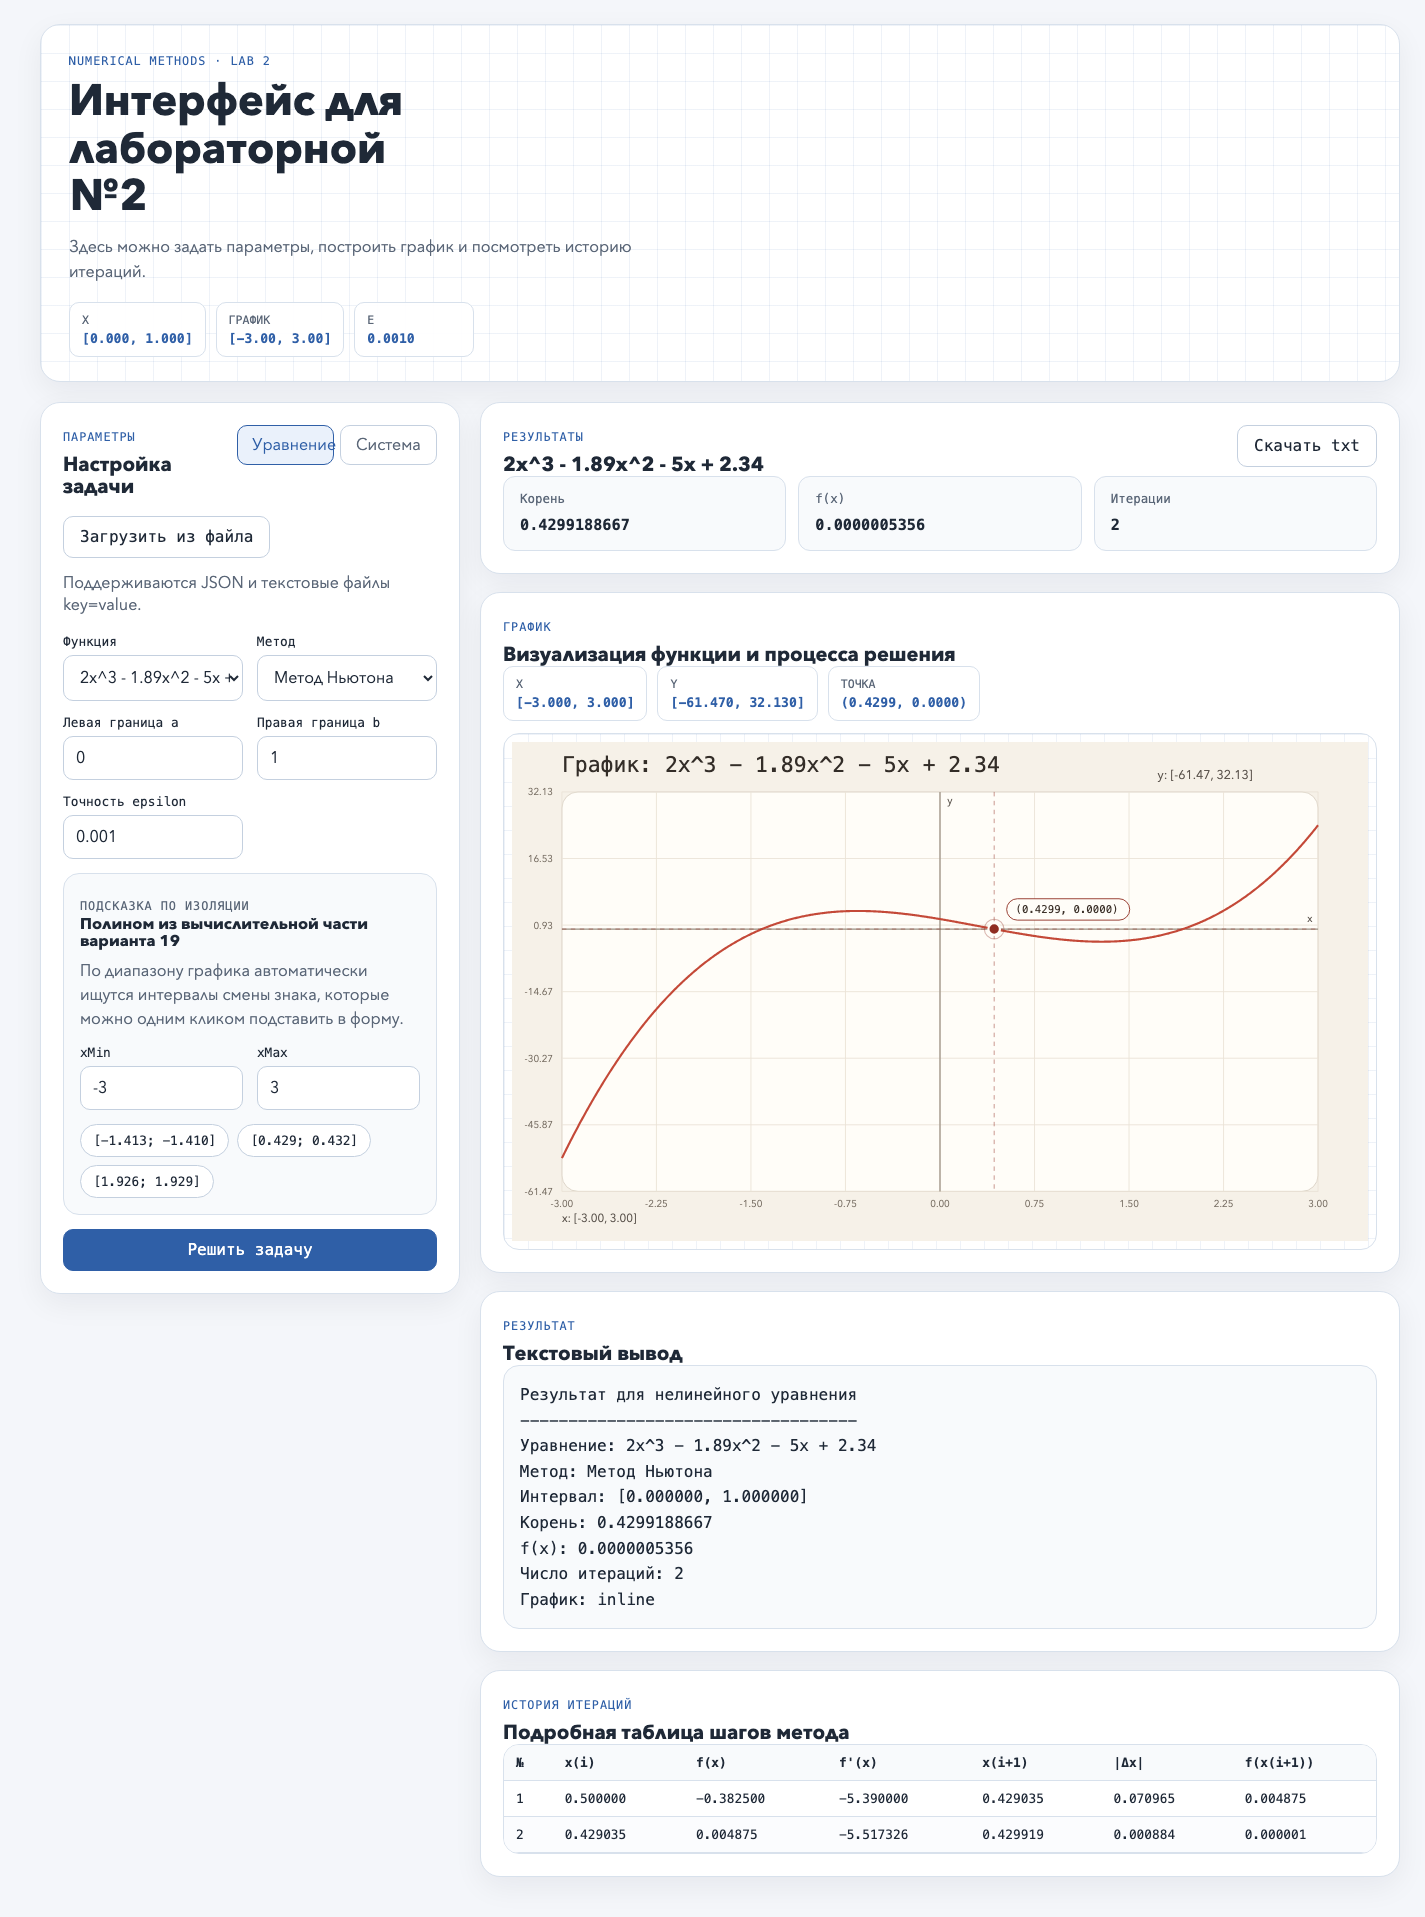
\includegraphics[width=0.96\textwidth]{output/screenshots/web-equation-result.png}
  \caption{Решение нелинейного уравнения в web-интерфейсе}
\end{figure}

\begin{figure}[H]
  \centering
  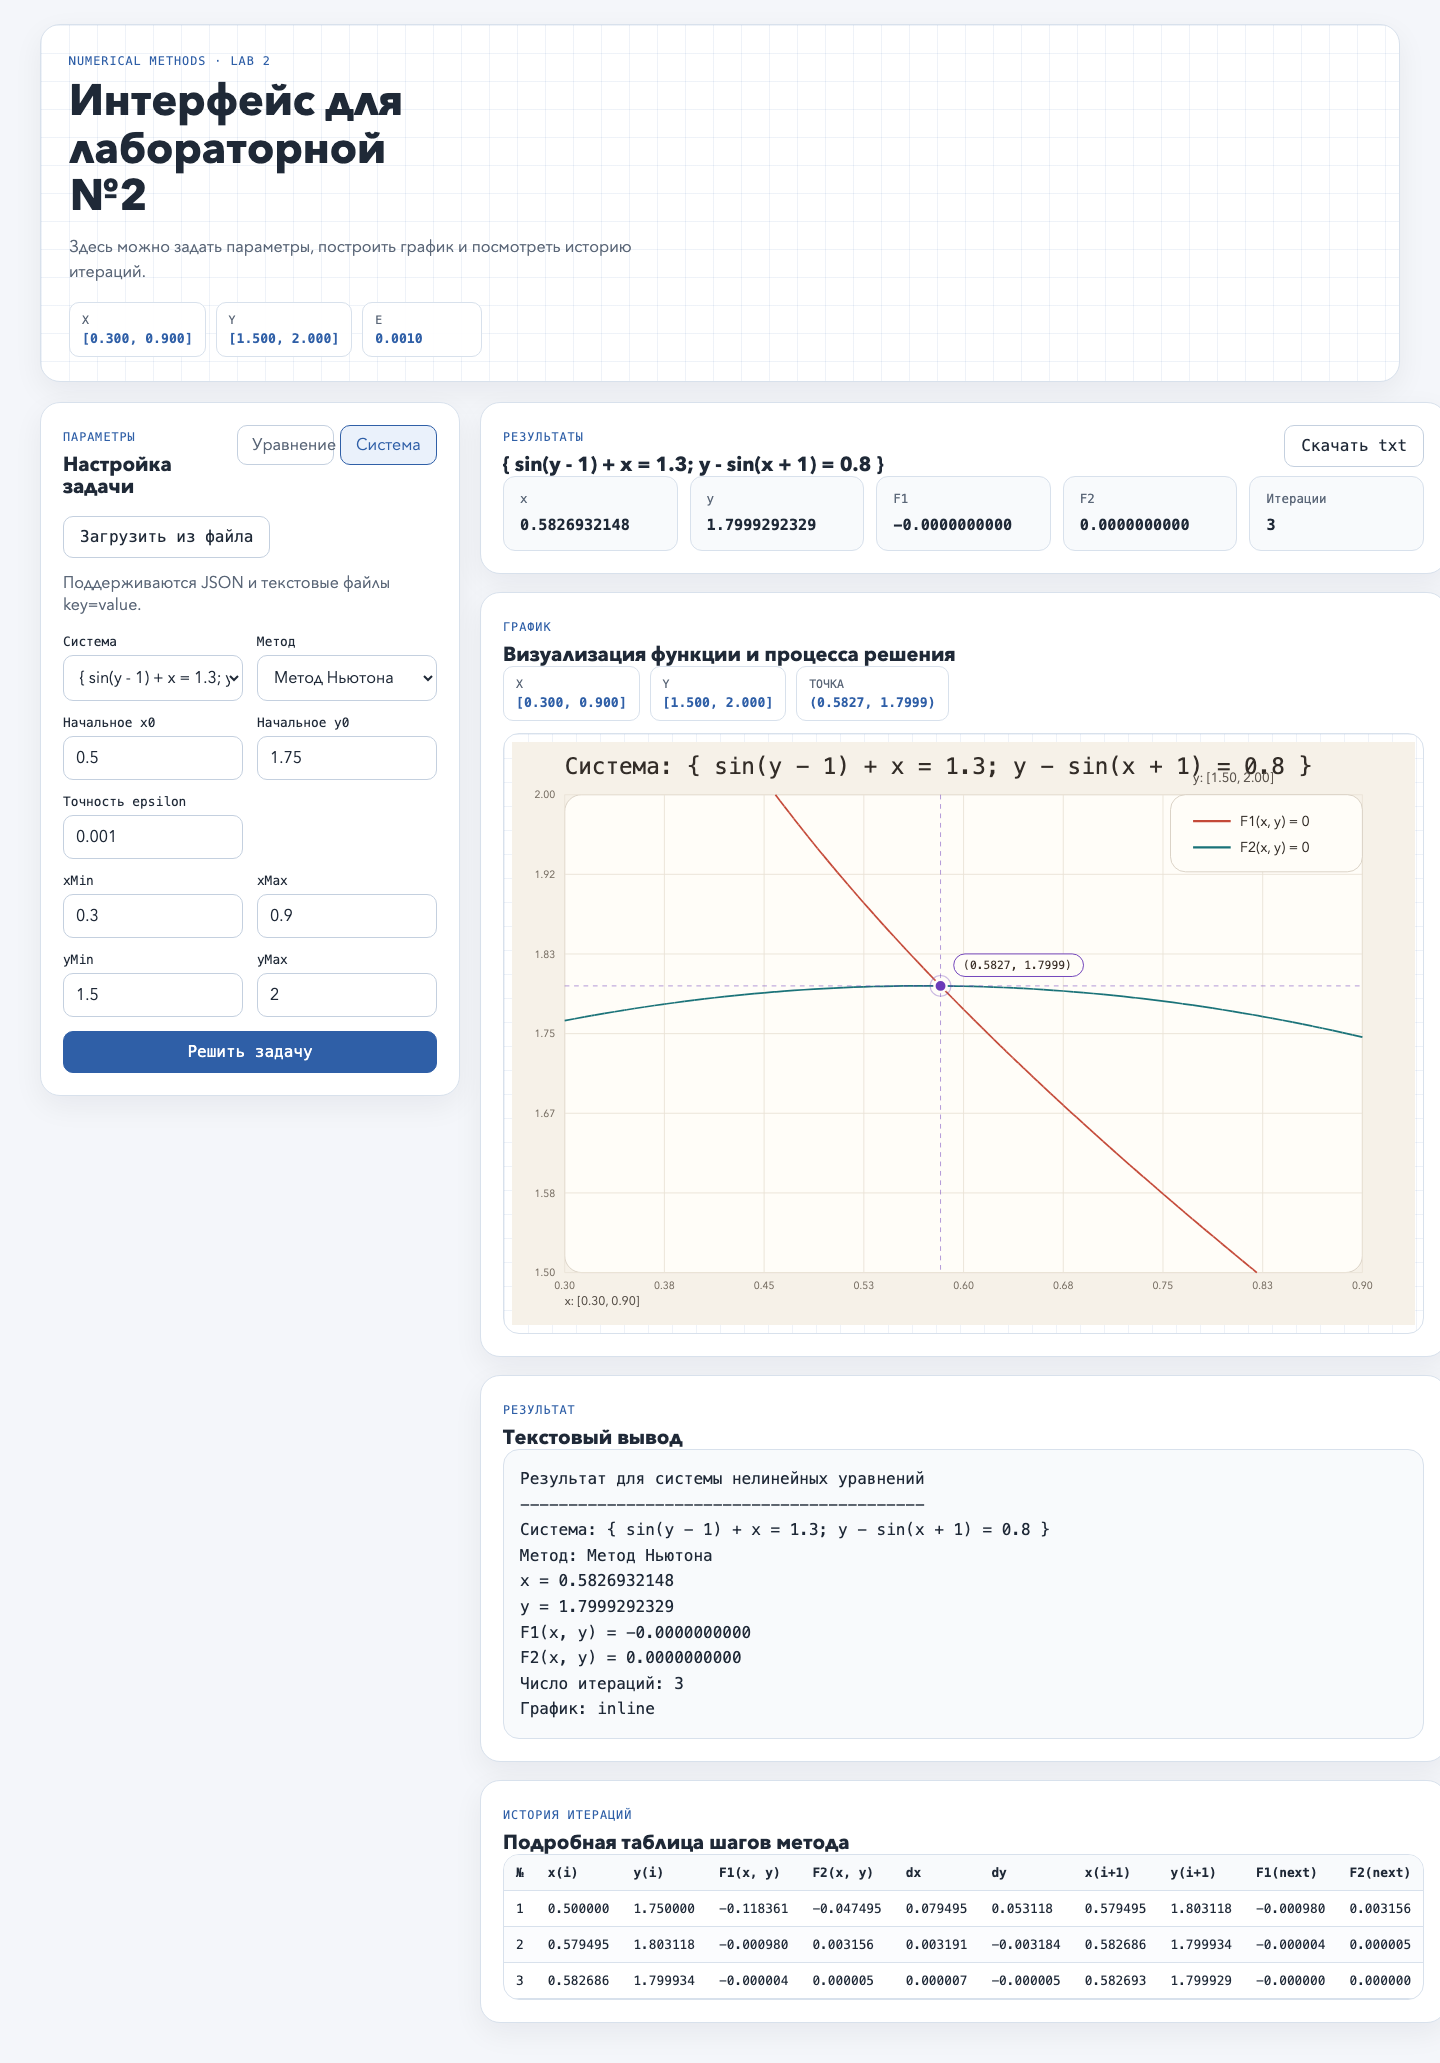
\includegraphics[width=0.96\textwidth]{output/screenshots/web-system-result.png}
  \caption{Решение системы нелинейных уравнений в web-интерфейсе}
\end{figure}

\section{Вывод}

В работе выполнено графическое отделение корней уравнения варианта 19, выбраны интервалы изоляции и получены приближённые значения корней с точностью $\varepsilon = 10^{-2}$. Для системы варианта 19 найдено решение $(x^*, y^*) \approx (0.583;\,1.800)$, невязки в найденной точке близки к нулю.

По таблице задания для варианта 19 в программе реализованы методы $2$, $3$, $5$ и $6$: хорд, Ньютона, простой итерации для уравнений и Ньютона для систем. В web-запуске метод Ньютона для уравнения сошёлся за $2$ итерации, метод Ньютона для системы --- за $3$ итерации. Метод хорд не требует производной, но зависит от выбора интервала и фиксированного конца. Метод простой итерации применим после проверки условия $q<1$; при нарушении этого условия программа выводит сообщение об ошибке. Web-интерфейс строит график, показывает таблицу итераций и сохраняет отображение графика при некорректном интервале.

\end{document}
